\section{EpToTester}
\label{sec:epto}
\eptotester is a framework using Docker and Docker Swarm. It is designed to ease the deployment of large scale distributed systems, more particularly \jgroups and \epto. We use \eptotester to assess the claims made in \autocite{matos2015epto}. Although \epto's implementation is written with benchmarking in mind, the code can be adapted for real applications with only minimal changes to the sources.
\subsection{Implementation}
We implement the network layer using UDP and our own PSS CYCLON operating on its own port to obtain a random view of peers. To obtain an initial random view, we contact an independent tracker implemented as a simple Python web server that keeps track of dead and alive nodes in the system. We want to emphasize that the tracker is not required. In practice it works well, but using a DHT is certainly a possibility.

We implement the payload as randomly generated UUIDs. We compare \epto to the deterministic total order algorithm SEQUENCER provided by \jgroups. We use \jgroups 3.6.11. When implementing \jgroups we use TCPGOSSIP \autocite{tcpgossip} provided by the \jgroups library instead of the traditional MULTICAST option to coordinate peers, as Docker services do not yet support MULTICAST. This is not a problem as in a real WAN \jgroups could not rely on MULTICAST.

The \epto simulation and theory is assuming we can have balls of infinite size. In practice, packet loss happens. We must therefore limit the ball size to a practical number. We use balls with a maximum size of \SI{1432}{\byte}. We choose this number as the default MTU on Ethernet is \SI{1500}{\byte}. We then subtract the bytes required for the IPv4 and UDP headers.
\subsection{Deployment}
 \begin{figure}[htp]
 	\centering
 	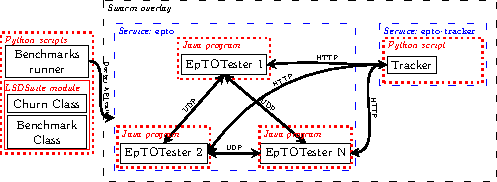
\includegraphics[width=\linewidth]{figures/complete-architecture.pdf}
 	\vspace{-2mm} 
 	\caption[Caption]{\eptotester architecture\footnotemark}
 	\vspace{-2mm} 
 	\label{fig:complete-architecture}
 \end{figure}
\footnotetext{This figure is partially inspired from a figure in \autocite{vaucher2016erasure}}
To deploy \epto effectively we need two different Docker Swarm services: one containing the tracker and one containing all \epto replicas. Both of these services use the same network overlay to communicate. This is achieved using Docker and especially the new Docker Swarm introduced in Docker 1.12. This lets us have a unified way of deploying our benchmarks locally or remotely on vastly different clusters with minimal modifications. Every benchmark is started through a Python script available on the master node. This script handles everything from starting benchmarks, scaling the cluster during a churn and collecting results. All \epto parameters are customizable by using options provided through this script.
Gradle\footnote{\href{https://gradle.org/}{https://gradle.org/}} is used to automate the project building. Finally, a script is provided to push the images to a repository accessible to the remote cluster and to push the benchmarking script on the master node. \jgroups deployment is much the same. The entire \eptotester architecture is shown in \autoref{fig:complete-architecture}.
\subsection{Fault Injection}
Our framework supports the ability to inject synthetic and real traces thanks to the work done in \autocite{vaucher2016erasure}. The synthetic churn provided by it was improved to support adding and removing nodes at the same time.
